% mainfile: ../../../../master.tex
\subsection{DNA quantification with Qubit\texttrademark DNA BR Assay Kit}
% The part of the label after the colon must match the file name. Otherwise,
% conditional compilation based on task labels does NOT work.
\label{task:20180227_cj2}
\tags{lab,dna,qnt}
\authors{cj}
%\files{}
%\persons{}
\sidenote{Qubit\texttrademark DNA BR Assay Kit \texttt{LOT:\#1835789} opened by Elísabet on 20170815.}

\begin{figure}[H] % position of the figure 
    \centering
    \caption{Illustration for the Qubit\texttrademark~ DNA BR assay}
    \label{fig:20180227_Qubit_dsDNA_BR}
    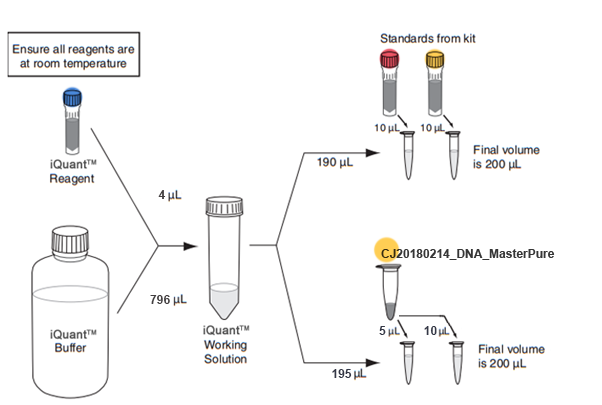
\includegraphics[width=0.8\textwidth]{graphics/schemas/20180215_Qubit_dsDNA_BR.png}
\end{figure}
\comment{It is exactly the same as what was done on the 20180215.}

In table \ref{tab:20180227_nuc_acid_qnt}, the quantities of DNA are calculted based on the volume left: I know I eluted my DNA with 2 x 100~\uL of Tris HCl buffer which makes it a total 200~\uL, then I used 2~\uL for the NanoDrop\cR measurments and finally I use 5~\uL and 10~\uL for the Qubit\texttrademark~ assay. Which means the volume left us 183~\uL. But based on these results, the original amount of DNA I was able to retrieve is -- at least -- 1542 ng, which is more 1~\textmu g of DNA!

\begin{table}[H]
\caption{Total DNA quantities in samples measured with Qubit\texttrademark~ DNA BR Assay Kit}
\label{tab:20180227_nuc_acid_qnt}
\centering
\begin{tabular}{l r r r r}
\toprule
Sample ID & \textmu g/mL & $V_f$ (mL) & m (\textmu g) & m (ng) \\ \midrule
\texttt{CJ20180227\_DNA\_AllPrep\_5} & 8.48 & 0.183 & - &  - \\
\texttt{CJ20180227\_DNA\_AllPrep\_10} & 8.16 & 0.183 & - & - \\
\texttt{CJ20180227\_DNA\_AllPrep\_5} & - & 0.183 & - & - \\
\texttt{CJ20180227\_DNA\_AllPrep\_10} & 7.71 & 0.183 & 1.410 & 1410.93 \\
\bottomrule
\end{tabular}
\end{table}

This is the highest DNA yield I have ever obtained (even higher than when I was working with more starting material!) which could mean that the bead beating is really helping to break cells.
